\documentclass{article}

% Language setting
% Replace `english' with e.g. `spanish' to change the document language
\usepackage[english]{babel}

% Set page size and margins
% Replace `letterpaper' with`a4paper' for UK/EU standard size
\usepackage[letterpaper,top=2cm,bottom=2cm,left=2.3cm,right=2.3cm,marginparwidth=1.75cm]{geometry}

% Useful packages
\usepackage[colorlinks=true, allcolors=blue]{hyperref}
\usepackage{color}
\usepackage{graphics} % for pdf, bitmapped graphics files
\usepackage{epsfig} % for postscript graphics files
\usepackage{newtxmath} % assumes new font selection scheme installed
\usepackage{times} % assumes new font selection scheme installed
\usepackage{cite}
\usepackage{amsmath,amssymb}
\usepackage{algorithmic}
\usepackage{subfigure}
\usepackage{textcomp}
\usepackage{xcolor}
\usepackage{booktabs}
\usepackage{multirow}
\usepackage{graphicx}
\usepackage{indentfirst}
\setlength{\parindent}{1.5em}
\usepackage{caption}
\captionsetup{font={small}}
% \usepackage{paralist}

\title{\LARGE \bf Response to Editor and Reviewers}
\date{}
\author{Authors of the manuscript}

\begin{document}
\maketitle

% \begin{abstract}
% Your abstract.
% \end{abstract}

\section*{Dear Editor and Reviews:}

Thank you very much for ......

(You can write the cover letter here and remember to tell the reviewers how the changes are highlighted.)
(At the end of the response file, you are suggested to list all the changes made in the revised manuscript.)

\section*{Response to Reviewer 1:}
\subsubsection*{1. 0   General Comments:}
The reviewer's general comments.

\subsubsection*{1. 1   Comment 1:}

The reviewer's first comment.  

I think you should add balabala.

\subsubsection*{-1. 1   Response 1:}
Thank you very much for your suggestion, we have added this into the revised manuscript which is shown as follows:

% \vspace{0.2cm}

\textbf{Changes are made in the xx paragraphs of section xx.}

Content in the revised manuscript  \textcolor{red}{with changes are highlighted in different color such as red.}



\subsubsection*{1. 2   Comment 2:}
The second comment of the review.

\subsubsection*{-1. 2   Response 2:}

\textbf{(1)} Thank you for your question, we

% \vspace{0.2cm}

\textbf{Changes are made in the xx paragraphs of section xx.}

Content in the revised manuscript  \textcolor{red}{with changes are highlighted in different color such as red.}

\section*{Response to Reviewer 2:}
\subsubsection*{2. 0   General Comments:}
General comments of review 2.

\subsubsection*{2. 1   Comment 1:}

The reviewer's first comment.

\subsubsection*{-2. 1   Response 1:}
\textbf{(1)} Thank you very much......

\textbf{Changes are made in the xx paragraphs of section xx.}

Content in the revised manuscript  \textcolor{red}{with changes are highlighted in different color such as red.}

If you need to add figures, try this:
\begin{figure}[!htbp]
\centering
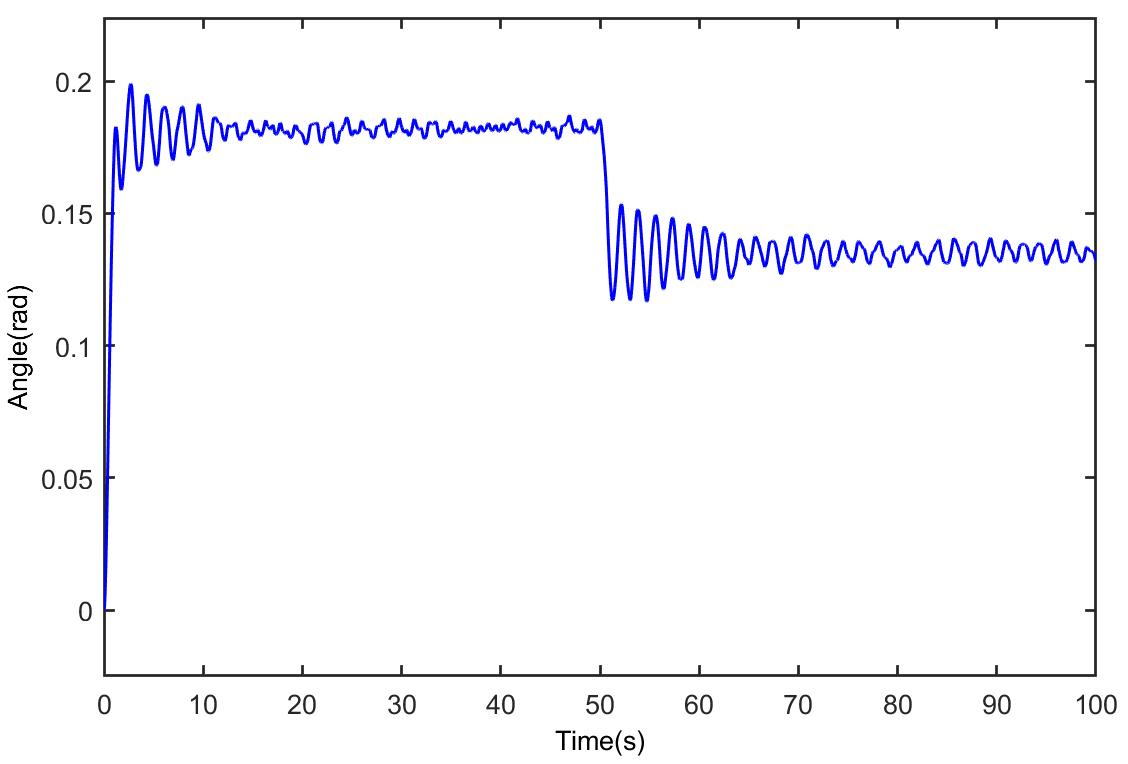
\includegraphics[width=7.5cm]{figure.jpg}
% \caption*{} %If you don't want the caption.
\caption{This is just a model.}
\label{fig1}
\notag % If you don't need the tag
\end{figure}

\section*{Response to Reviewer 3:}
\subsubsection*{3. 0   General Comments:}
This paper describes......



\section*{List of Major Changes.}
\begin{itemize}
    \item{1.} We have ......
    \item{2.} We have ......
    \item{3.} ......
    \item{4.} ......
    \item{5.} We ......

\end{itemize}

You are also suggested to provide a version of the manuscript with changes highlighted. A easier way is to use Adobe Acrobat DC and paste the manuscript after the response. Best wishes!!! You can do it!!!!!!

\end{document}